\documentclass[a4paper,10pt]{report}
\usepackage[utf8]{inputenc}
\usepackage{color}
\usepackage{colortbl}
\usepackage{graphicx}
% Title Page
%\title{}
%\author{}

\definecolor{Gray}{gray}{0.8}
\definecolor{lightGray}{gray}{0.925}

\newcolumntype{A}{>{\columncolor{Gray}}c}
\newcolumntype{B}{>{\columncolor{Gray}}l}

\begin{document}
%\maketitle
\begin{titlepage}

\begin{center}
\begin{tabular}{|A|}
\hline
\\
\\
\\
\bfseries \Huge \quad \quad \quad  Pflichtenheft   \quad \quad \quad
\\
\\
\Large zum Softwareprojekt\\
\Large (Prof. Steinbach)\\
\\
\\
\hline
\end{tabular}
\end{center}

\vspace{3,5mm}

\begin{center}
\begin{tabular}{|A|}
%Hier Projektnamen einfügen.
%Bei Bedarf die \quad entfernen, sie dienen nur der einheitlichen Breite der Tabellen
\hline
\\
\\
\bfseries \Large \quad \quad \quad Struktogrammeditor (42) \quad \quad \quad
\\
\\
\\
\\
\hline
\end{tabular}
\end{center}

\vspace{9mm}

\bfseries \large Angaben zu den am Projekt beteiligten Studenten:

\begin{center}
\begin{tabular}{|c|l|l|l|l|}
%Hier Mitglieder der Projektgruppe eintragen. Vor jeden Namen ein \normalsize setzen; wird die Tabelle durch lange Namen zu groß \normalsize durch \small ersetzen
\hline
\rowcolor{Gray}\normalsize &\normalsize Name, Vorname &\normalsize Mat.-Nr. &\normalsize Studiengang &\normalsize Email-Adresse \\
\hline
\rowcolor{lightGray}\normalsize 1. &Jonas Toth &57319 &BAI &Jonas.Toth@student.tu-freiberg.de\\
\hline
\rowcolor{Gray}\normalsize 2. &Christian Sacher &57406 &BAI &Christian.Sacher@student.tu-freiberg.de \\
\hline
\rowcolor{lightGray}\normalsize 3. &Martin Plank&57464 &BAI &plank-martin@web.de  \\
\hline

\end{tabular}
\end{center}

\vspace{10mm}

\begin{center}
\begin{tabular}{|BB|}
\hline
\bfseries \large Best\"{a}tigt durch Prof. Steinbach & \quad \quad \quad \quad \quad \quad \quad \quad \quad \\
\bfseries \large Datum, Unterschrift &
\\
\hline
\end{tabular}
\end{center}

\end{titlepage}
%\begin{abstract}
%\end{abstract}

\newpage
\renewcommand{\thesection}{\arabic{section}}

\tableofcontents
\newpage
\section{Zielbestimmung}
Ziel des Softwareprojektes ist es, ein Programm zur Erzeugung und Visualisierung von Struktogrammen zu erstellen. 
Mit dessen Hilfe sollen Programmieranf\"{a}nger ein Tool in der Hand haben um Algorithmen und Programme systematisch zu verstehen und entwickeln.
\subsection{Musskriterien}
\begin{itemize}
\item Struktogramm dynamisch erstellen
\item GUI zur Benutzerfreundlichen Bedienung
\item Baumstruktur des Struktogramms visualisieren
\item Speichern und Laden von Struktogrammen
\item
\end{itemize}
\subsection{Wunschkriterien}
\begin{itemize}
\item XML Generierung aus Struktogrammen. Dies soll zum vereinfachten exportieren dienen und geht damit mit speichern und laden einher.
\item Visualisierung des Programmablaufes
\item Export zu gängigen Bildformaten
\end{itemize}
\subsection{Abgrenzungskriterien}
\begin{itemize}
\item Es soll kein funktionierendes Programm aus dem Struktogramm generiert werden.
\end{itemize}

\section{Produkteinsatz}
\subsection{Anwendungsbereiche}
Das Programm soll Leuten helfen, die neu ins Programmieren oder in die Informatik einsteigen. Aber vor allem soll es das algorithmische Denken veranschaulichen.
\subsection{Zielgruppen}
\begin{itemize}
\item Schüler und Studenten
\item Menschen die sich mit Informatik beschäftigen
\end{itemize}
\subsection{Betriebsbedingungen}
\begin{itemize}
\item Das Programm soll auch von Anfängern benutzt werden können
\item Das Programm muss nicht beobachtet werden da es nur auf Input reagiert
\item Das Programm soll ohne Laufzeitbegrenzung sein
\end{itemize}
\section{Produktumgebung}
\subsection{Software}
\begin{itemize}
\item Windows 7 und höher
\item .Net
\end{itemize}
\subsection{Hardware}
\begin{itemize}
\item Maus
\item Tastatur
\item Desktop
\item >200MB Ram >1GHZ CPU
\end{itemize}
\subsection{Orgware}
\begin{itemize}
\end{itemize}
\subsection{Produktschnittstellen}
\begin{itemize}
\item NA
\end{itemize}

\section{Produktfunktionen}
\begin{itemize}
\item /F10/ Struktogram auf einzelnen Blöcken zusammen setzen
\item /F20/ Löschen der Eingegeben Daten (abbrechen)
\item /F30/ Auswahl welcher Logische Block (if, loop, sequenz)
\item /F40/ bestehenden Block löschen
%Dateiverwaltung:
\item /F50/ Neue Datei erstellen
\item /F60/ Datei speichern + speichern als
\item /F70/ Datei öffnen
\item /F80/ exportieren (als Bild)
\item /F90/ Drucken?!
%Ansicht
\item /F100/ Baumdiagrammansicht an/aus schalten
\item /F110/ Output an/aus schalten
\item /F120/ Normalmodus anschalten (macht Output und Baumdiagramm aus)
\end{itemize}

\section{Produktdaten}
\begin{itemize}
\item /D10/ Baumdiagramm bzw. Daten des Struktograms (Graphen speichern)
\end{itemize}
\section{Produktleistungen}
\begin{itemize}
\item /L10/ Das Programm soll ohne lange Wartezeiten sein
\end{itemize}
\section{Benutzeroberfläche}
\begin{figure}[h!]
  \caption{}
  \centering
    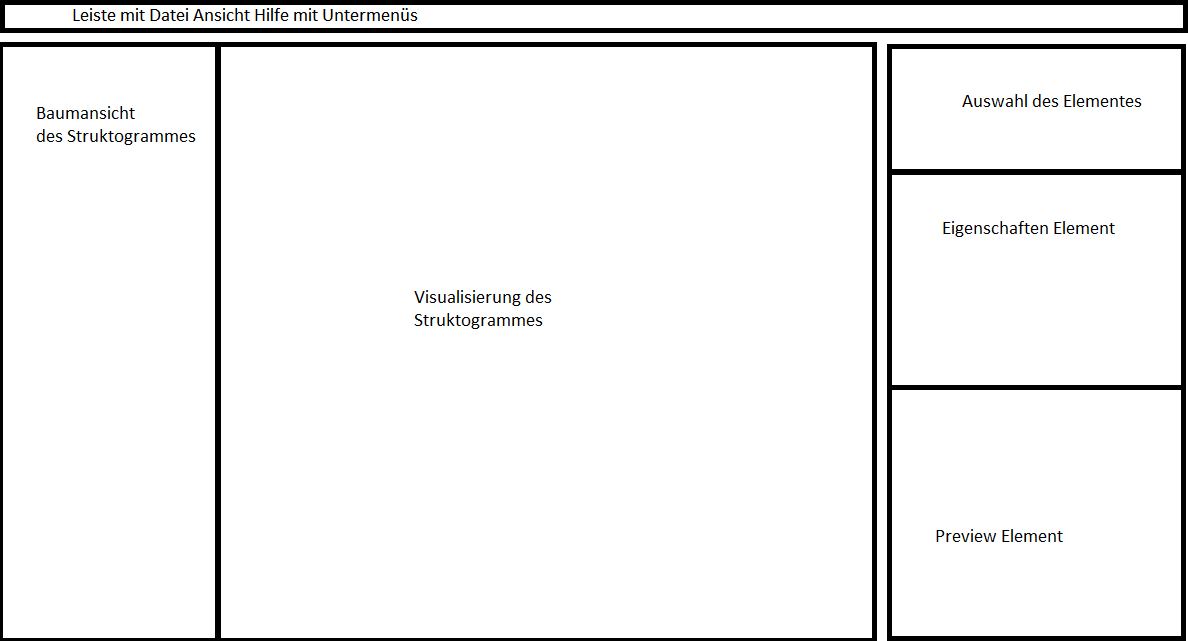
\includegraphics[width=1.3\textwidth]{gui-skizze.png}
\end{figure}
Baumstruktur Anzeigen von allen Elementen innerhalb des Struktogrammes in hieraischer Form.
Preview Anzeigen des Elementes welches hinzugefügt werden soll.
Visualisierung Anzeigen des gesamten Struktogrammes

\section{Qualitätszielbestimmung}

\begin{center}
  \begin{tabular}{| l | l | l | l | l |}
    \hline
   	 Produktqualität & Sehr Gut & Gut  & Normal & Nicht Relevant \\ \hline
    	 Funktionalität &   &  x &  & \\ \hline
 	 Zuverlässigkeit & x  &   &  & \\ \hline
 	Benutzbarkeit &   &  x &  & \\ \hline
      	 Effizienz &   &  x &  & \\ \hline
      	 Änderbarkeit &   &  &  x & \\ \hline
      	Übertragbarkeit &   &   &  & x \\ \hline
  \end{tabular}
\end{center}


\section{Globale Testszenarien/Testfälle}
\begin{itemize}
\item  Erstellen eines Struktograms
\item  Laden/Speichern eines Struktograms
\item  Exportieren eines Struktograms (Wunschkriterium)
\end{itemize}
\section{Entwicklungsumgebung}
\subsection{Software}
\begin{itemize}
\item Visual Studio 2015
\item git in Kombination mit github.com
\end{itemize}
\section{Ergänzungen}
\section{Verteilung der Aufgaben zwischen den Projektteilnehmer}
F10-F40 Martin Plank
F50-F70 Christian Sacher
F80-F120 Jonas Toth


\section{Glossar}
\begin{itemize}
% u read here https://de.wikipedia.org/wiki/Nassi-Shneiderman-Diagramm
	\item Sequenz -> einfache Anweisung
	\item Alternative
	\item Alternative Verzweigung
	\item Fallauswahl
	\item Zählergesteuerte Schleife
	\item Kopfgesteuerte Schleife
	\item Fußgesteuerte Schleife
	\item Endlosschleife
	\item Aussprung
	\item Aufruf
\end{itemize}
\end{document}
